\item Złożenie zamówienia \\
 

 Opis słowny - jest to główny przypadek użycia, będący podstawową jednostką
 działania w niemal każdym sklepie internetowym. Złożenie zamówienia rozpoczyna
 się w momencie wyboru interesujących klienta towarów. Następnie zostaje on
 przekierowany do ekranu końcowego, gdzie wybiera sposób płatności i akceptuje
 zamówienie. Następnie zostaje do klienta wysłany e-mail potwierdzający
 
 \begin{longtable}{|p{5cm}|p{7cm}|}
 	\hline
	\textbf{Aktor} & Klient \\
	\hline
	\textbf{Warunki początkowe} & Klient zalogowany \\
	\hline
	\textbf{Opis przebiegu interakcji} & Wybór towarów, wybór sposobu płatności,
	akceptacja zamówienia \\
	\\
	\hline
	\textbf{Sytuacje wyjątkowe} & Użytkownik niezalogowany, użytkownik wycofuje się
	z  transakcji
	\\
	\hline
	\textbf{Warunki końcowe} & Nowe zamówienie w systemie \\
	\hline
 \end{longtable}


\item Złożenie zamówienia - scenariusz główny \\ 
  \begin{tabularx}{\linewidth}{ c X }
  Aktor: & Klient \\
  \end{tabularx}
  \begin{enumerate}
    \item Klient uruchamia stronę internetową sklepu i wyszukuje interesujące go
    produkty
    \item W momencie znalezienia pasującego produktu użytkownik wybiera opcję
    dodania do koszyka
    \item Po zakończeniu wyszukiwania użytkownik wybiera opcję przejścia do kasy
    \item System sprawdza, czy użytkownik jest zalogowany. 
    \item System sprawdza, czy użytkownik jest stałym klientem. Jeśli tak,
    dolicza rabat do ustalonej ceny (do sumy cen poszczególnych produktów)
    \item Użytkownik wybiera sposób płatności
    \item System dodaje do wcześniej ustalonej ceny koszty wynikające ze sposobu
    płatności
    \item Użytkownik wybiera sposób dostawy (poczta, kurier, odbiór osobisty
    itp.)
    \item System dodaje do ceny koszty wynikające ze sposobu dostawy
    \item Użytkownik, po sprawdzeniu wszystkich danych, decyduje się na złożenie
    zamówienia - po tym momencie nie może już ono być cofnięte
    \item System wysyła do użytkownika e-mail potwierdzający wraz z przewidywaną
    datą realizacji zamówienia
		
  \end{enumerate} 
  
  
  \item Złożenie zamówienia - scenariusz alternatywny - klient nie klika w linka
aktywacyjny
   \begin{tabularx}{\linewidth}{ c X}
	Aktor: & Klient \\
  	\end{tabularx}   
  	\begin{enumerate}
  	  \item Kroki 1-3 scenariusza głównego
  	  \item Jeśli użytkownik jest niezalogowany, system rozpoczyna procesowanie
  	  przypadku użycia Logowanie Do Systemu
  	  \item Po poprawnym zalogowaniu procesowanie przypadku użycia odbywa się jak
  	  w punktach 5-11
  	\end{enumerate}
  	
  	
  	\item Złożenie zamówienia - scenariusz alternatywny - klient rezygnuje z
  	zamówienia aktywacyjny
   \begin{tabularx}{\linewidth}{ c X}
	Aktor: & Klient \\
  	\end{tabularx}   
  	\begin{enumerate}
  	  \item Kroki 1-9 scenariusza głównego
  	  \item Użytkownik, po przeglądnięciu podsumowania całego zamówienia, nie
  	  decyduje się na złożenie zamówienia.
  	  \item System usuwa wszystkie dane tymczasowe z przeglądarki internetowej
  	  \item Pojawia się okno startowe sklepu internetowego
  	\end{enumerate}
  	
  	
   	
\begin{figure}[H]
    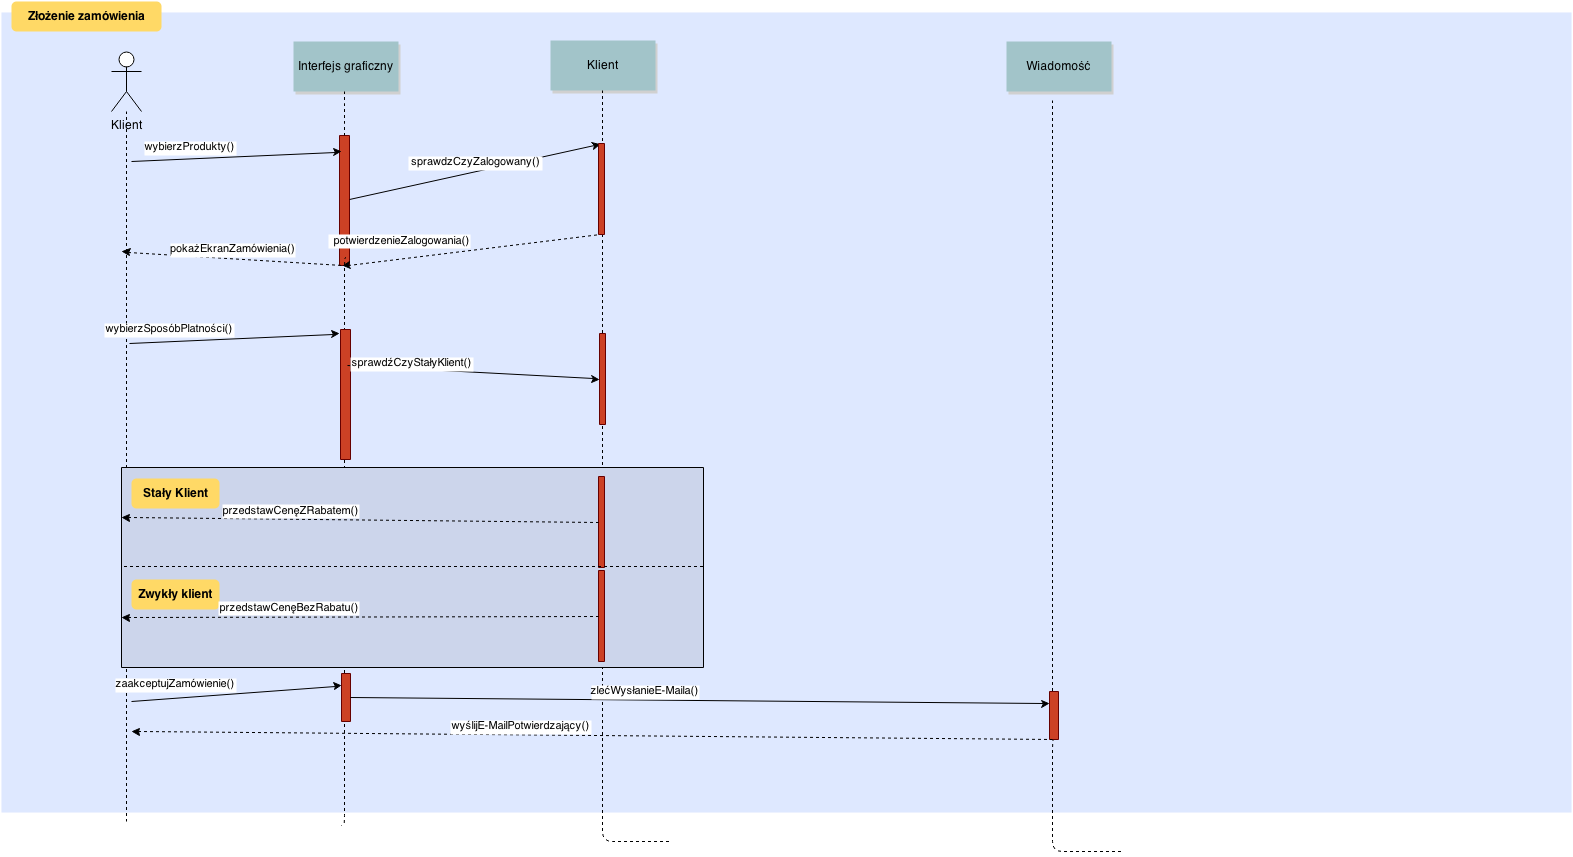
\includegraphics[width=\textwidth,
    height=0.5\textheight]{graphics/UseCase/Klient/ZlozenieZamowieniaSD.png}
  \caption{Diagram sekwencji dla przypadku użycia Złożenie Zamówienia -
  scenariusz główny}
\end{figure}